\chapter{Mini-KaZaA Client}
Oltre che di un Bootstrap server, la rete Mini-KaZaA si basa su un client che gli utenti possono usare per accedere alla rete e poter condividere e scaricare file.
\section{Mini-KaZaA Client in generale}
Mini-KaZaA client presenta tutte le funzionalità che consentono una condivisione peer to peer dei contenuti.
Ogni client al primo avvio chiede all'utente, tramite un comodo pannello, di scegliere il \emph{ruolo} da interpretare all'interno della rete.

Chi ha più risorse da mettere a disposizione e una banda di comunicazione più ampia può scegliere di essere un Super Node, che oltre a condividere e scaricare, ha la funzione di smistare le query nella rete e accettare richieste direttamente dagli Ordinary Node \emph{figli}. Chi ha meno risorse da mettere a disposizione può scegliere di essere un semplice Ordinary Node.

\section{Il codice di Mini-KaZaA client}
Il codice di Mini-KaZaA client è distribuito in tre diverse librerie:
\begin{itemize}
 \item \textbf{lpr.minikazaa.minikazaaclient}: questa libreria contiene classi comuni a tutti e due i tipi di client dal punto di vista logico. L'esempio più evidente è la classe \verb|MainGui.java|.
 \item \textbf{lpr.minikazaa.minikazaaclient.ordinarynode}: questa libreria contiene le classi che loogicamente appartengono al tipo di client Ordinary Node, ma che, all'occorrenza, possono essere importate anche da un Super Node.
 \item \textbf{lpr.minikazaa.minikazaaclent.supernode}: questa libreria, infine contiene tutte le classi che servono a un supernodo per funzionare e che appartengono a questo logicamente. Alcune di queste classi, come per esempio \verb|SupernodeCallbacksInterface.java|, vengono utilizzate anche dagli ORdinary Node.
\end{itemize}

Questa suddivisione è puramente logica visto che i due tipi di client differiscono solo per alcune caratteristiche.

Si è preferito dividere anche le classi che contengono gli stessi task per i SN e per gli ON per poter meglio gestire il codice e renderlo più modulare.
Un esempio è rappresentato dalle classi \verb|OrdinarynodeWorkingThread.java| e \verb|SupernodeWorkingThread.java| che hanno lo stesso compito, ma, che piuttosto che complicare con una serie di 
\begin{verbatim}
if <condizione> then 
	<blocco> 
else 
	<blocco>|
\end{verbatim}
si è preferito separare in due classi distinte.

Passiamo ora a una presentazione più particolareggiata del codice comune a Super Node e Ordinary Node.

\section{Le strutture dati comuni}
Per lo sviluppo di Mini-KaZaA è stato necessario predisporre una serie di strutture dati che tutto il software
utilizzi per condividere informazioni.

All'interno del package \verb|lpr.minikazaa.minikazaaclient| troviamo le seguenti classi che rappresentano strutture dati comuni a SN e ON:
\begin{itemize}
 \item \verb|NodeConfig.java|
 \item \verb|Query.java|
 \item \verb|Answer.java|
 \item \verb|SearchField.java|
 \item \verb|Download.java|
 \item \verb|DownloadRequest.java|
 \item \verb|DownloadResponse.java|
\end{itemize}

Guardiamo cosa si nasconde all'interno di ognuna di queste classi.

\subsection{NodeConfig.java}
La classe \verb|NodeConfig.java| contiene i seguenti attributi:
\newline
\begin{lstlisting}
private String user_name;
private int port;
private String bootstrap_address;
private int max_conn;
private int ttl;
private boolean is_sn;

//Calcolato all'avvio
private String my_address;
\end{lstlisting}

Questi attributi sono i campi che l'utente inserisce nel form al primo avvio del programma e contengono le informazioni di configurazione del nodo. 

\subsection{Query.java}\label{sec:query}
La classe \verb|Query.java| viene utilizzata dal client Mini-KaZaA per l'invio di richieste di file nella rete.

Contiene diversi attributi per i quali ci sono i metodi \verb|set| e \verb|get|. Questa classe inoltre implementa
le interfacce \verb|Serializable| e \verb|Cloneable|.
La prima serve per poter inviare su rete come flusso di byte l'oggetto \verb|Query|. La seconda invece serve per poter
copiare un'istanza dell'oggetto \verb|Query| in una seconda istanza.
\newline
\begin{lstlisting}
//Espressione regolare della query
private String body_q;

//Query di risposta
private Answer body_a;

//Notifica a un supernodo di avere
//file da condividere
private OrdinarynodeFiles body_f;

//Sorgente di una query
private NodeInfo id_origin;

//NodeInfo del mittente
private NodeInfo sender;

//NodeInfo del destinatario
private NodeInfo receiver;

//Time to live della query
private int ttl;

//Id della query attribuito dall'origine
private int id;
\end{lstlisting}

La classe \verb|Query| ha tre gruppi di attributi.Un primo gruppo descrive il contenuto della query e di conseguenza
il tipo di query. Un secondo gruppo serve per identificare i soggetti coinvolti nello scambio della query stessa.
Il terzo gruppo contiene invece parametri per l'identificazione della query. 

Analizziamo uno ad uno questi parametri per capire meglio come funzionano le query in Mini-KaZaA.
\begin{itemize}
 \item \verb|body_q|:
il vero corpo della query di richiesta di un file. \`{E} una stringa che contiene un
espressione regolare che il client Mini-KaZaA riesce a interpretare;

 \item \verb|body_a|:
la parte dell'oggetto \verb|Query| che contiene la risposta a una determinata richiesta. Analizzaremo la classe
\verb|Answer| successivamente;

 \item \verb|body_f|:
questo campo viene riempito da un ON che vuole inviare al proprio SN la sua lista di file per metterli a disposizione
di tutti;

 \item \verb|id_origin|:
per ogni query deve essere nota l'origine dalla quale proviene la query stessa per poi poterla correttamente fermare
al punto giusto e farla ritornare al mittente. Questo è il compito del campo \verb|id_origin|;

 \item \verb|sender|: 
questo campo indica uno dei due soggetti che sono impegnati in un singolo scambio di query, il nodo da cui parte;

 \item \verb|receiver|:
questo campo indica il nodo a cui deve arrivare la query in uno scambio;

 \item \verb|ttl|:
questo campo sta per \emph{Time To Live} e indica il numero di scambi per il quale la query deve continuare a esistere.
Serve principalmente per evitare che si creino dei cicli infiniti di scambio della query ottenendo quindi una valanga
di dati ridondanti con conseguente intasamento della rete;

 \item \verb|id|:
ogni nodo può inviare più query alla volta nella rete e il compito di questo campo è di identificare univocamente la
query presso il suo nodo origine.
\end{itemize}

\subsection{Answer.java}
La classe \verb|Answer.java| contiene i file che possono corrispondere ai criteri di una ricerca. 

\`{E} una classe molto semplice ma molto utile per indicizzare rapidamente i file.

Ecco il codice nel quale vengono dichiarati gli attributi della classe.
\newline
\begin{lstlisting}
//File che corrispondono a una query
private ArrayList <OrdinarynodeFiles> files;

//Id della query assegnato dall'origine
private int id;
\end{lstlisting}

L'attributo \verb|files| è una lista di OrdinarynodeFiles, Sezione \ref{sec:on_files}.

La classe \verb|Answer.java| viene utilizzata 

L'attributo \verb|id| richiama semplicemente l'id univoco della query di cui fa parte l'oggetto \verb|Answer|.

\subsection{SearchField.java}
La classe \verb|SearchField.java| viene utilizzata dal client Mini-KaZaA per tenere in memoria tutti i risultati
associati a una richesta di file.
Da uno di questi campi poi vengono estratte le informazioni per eventuali download di file.

Anche questa classe è piuttosto semplice poichè funziona da appoggio alla rappresentazione grafica e per snellire
la quantità di informazioni da tenere in memoria per l'utente.

Il codice che descrive gli attributi della classe è il seguente:
\newline
\begin{lstlisting}
//File owner
private NodeInfo owner;

//File descriptor
private MKFileDescriptor file;
\end{lstlisting}

Con queste due semplici informazioni è possibile sia risalire al proprietario, compreso l'indirizzo ip da contattare
per il download, sia ottenere tutti i metadati del file da scaricare\footnote{I download così come le ricerche vengono
effettuati mediante l'hash univoco md5 che tratteremo nella Sezione \ref{sec:md5}}.

\subsection{Download.java}
La classe \verb|Download.java| serve al client Mini-KaZaA per indicizzare i downloads che si effettuano. Questa classe si distingue da \verb|SearchField.java| perchè mantiene anche il numero di byte già scaricati.
\newline
\begin{lstlisting}
private MKFileDescriptor file_to_download;
private long downloaded_bytes;
private String downloader_path;

public Download(MKFileDescriptor file){

	this.file_to_download = file;
	this.downloaded_bytes = 0;

	//Directory di default
	this.downloader_path = "./downloads/";
}
\end{lstlisting}

Gli attributi della classe \verb|Download.java| sono quelli elencati nel listato mostrato appena sopra.
\verb|file_to_download| identifica il file che si sta scaricando tramite il codice hash \emph{md5}. Viene anche usato il nome del file, salvato all'interno di \verb|MKFileDescriptor|, per poter comporre il path assoluto con l'attributo \verb|downloader_path|. I \verb|downloaded_bytes| invece indicano, quanta parte di file è stata già scaricata dalla rete.

\subsection{DownloadRequest.java}
La classe \verb|DownloadRequest.java| viene utilizzata dal client Mini-KaZaA per richiedere file da scaricare al nodo che lo possiede.
Si compone dei seguenti attributi:
\newline
\begin{lstlisting}
//File da scaricare
private String file_request;

//Sorgente della richiesta
private NodeInfo request_source;
\end{lstlisting}

\subsection{DownloadResponse.java}
Il client Mini-KaZaA fa un uso particolare della classe \verb|DownloadResponse.java|. Essa viene infatti usata sia per inizializzare e terminare una comunicazione, sia come ``mezzo di trasporto'' delle varie parti di un file.

Vediamo innanzitutto quali attributi include questa classe:
\newline
\begin{lstlisting}
//byte che compongono una parte di 
//un file
private byte [] part;

//File inviato
private String file;
\end{lstlisting}
Mini-KaZaA ``spezzetta'' il file da inviare in piccoli pacchetti da 4Kb che vengono inseriti all'interno dell'array \verb|part|.
\verb|file| invece contiene l'md5 del file che viene inviato. Questa classe, e la combinazione dei suoi paramtri, permettono a Mini-KaZaA di controllare l'inizio di una comunicazione, la fine della stessa, e tutti gli invii intermedi di byte.
Vedremo meglio come funziona lo scambio di file all'interno della Sezione \ref{sec:scambio}

\section{Il percorso di una query}
Nella sezione \ref{sec:query} abbiamo visto di cosa si compone la classe \verb|Query.java|. Ora vediamo come viene utilizzata dal client nello scambio di richieste.

Ogni query di ricerca di file comincia con l'input dell'utente tramite un apposita formdi cui parleremo nella Sezione \ref{sec:grafica}.
Viene così generato un oggetto di tipo query con il seguente frammento di codice:
\begin{lstlisting}
Query q = new Query();
q.setId(this.my_num);
q.setSender(this.my_infos);
q.setOrigin(this.my_infos);
q.setAskingQuery(this.search_tf.getText());
q.setTTL(this.my_conf.getTimeToLeave());
\end{lstlisting}
Questo oggetto viene così inviato nella rete attraverso i SN.
Ogni SN leva un'unità di \emph{TTL} alla query e la rimbalza nella rete.

La gestione del percorso di una query è affidata completamente alla classe \verb|SupernodeTCPWorkingThread.java| e ne parleremo in Sezione \ref{sec:smistamento_delle_query}.
Quest'operazione è comune ai due tipi di client, ma contiene delle ovvie differeze, dovute alla natura dei vari nodi, che spiegheremo più avanti.

\section{La classe SupernodeList.java}
La classe \verb|SupernodeList.java| è una delle classi principali del progetto. Essa infatti mantiene un elenco dei SN presenti sulla rete.
Essa in realtà è molto utile per indicizzare insiemi di nodi di qualsiasi tipo, difatti il Bootstrap server utilizza proprio questa classe per le sue liste di nodi.

Come si può vedere dal seguente listato:
\begin{lstlisting}
private ArrayList<NodeInfo> sn_list;
private ArrayList<NodeInfo> sub_set_list;

public SupernodeList() {
	this.sn_list = new ArrayList();
	this.sub_set_list = null;
}
\end{lstlisting}

la classe \verb|SupernodeList.java| è composta da due attributi:
\begin{itemize}
 \item \verb|sn_list|:
un'\emph{ArrayList} di \verb|NodeInfo| utilizzata per tenere in memoria \emph{tutti} i nodi della rete;

 \item \verb|sub_set|:
una seconda \emph{ArrayList} di \verb|NodeInfo| utilizzata di volta in volta per memorizzare un sottoinsieme di nodi vicini e convenienti da contattare.
\end{itemize}


\begin{lstlisting}
public synchronized void 
refreshPing(InetAddress ia, int port, long new_ping) {
	for (NodeInfo n : sn_list) {
		//Confrontiamo l'indirizzo del nodo estratto 
		//con quello passato come parametro del metodo
		if (n.getIaNode().toString().equals(ia.toString())) {
			if (n.getDoor() == port) {
				n.setPing(new_ping);
			}
		}
	}
}

public synchronized void refreshPing() {
	//Thread pool
	ThreadPoolExecutor my_thread_pool =
		new ThreadPoolExecutor(
			10, 15, 50000L, 
			TimeUnit.MILLISECONDS,
			new LinkedBlockingQueue<Runnable>());
	
	if (this.sn_list.size() >= 1) {
		for (NodeInfo n : sn_list) {
			NodePing pinging = 
				new NodePing(
					n.getIaNode(), 
					n.getDoor(), 
					this);

			my_thread_pool.execute(pinging);
		}
	}
	my_thread_pool.shutdown();

	this.setChanged();
	this.notifyObservers();
}
\end{lstlisting}

\begin{lstlisting}
public synchronized void 
subSet(int set_size, long threshold) {
	ArrayList<NodeInfo> neighbors = new ArrayList();

	for (NodeInfo n : this.sn_list) {
		if (n.getPing() != -1) {

			if (n.getPing() <= threshold) {
				neighbors.add(n);
				if (neighbors.size() == set_size) {
					this.sub_set_list = neighbors;
				}
			}
		}
	}

	this.sub_set_list = neighbors;
}

public synchronized ArrayList<NodeInfo> getSubSet() {

	if (this.sub_set_list == null) {
		subSet(10, 100);
	}

	return this.sub_set_list;
}

public synchronized NodeInfo getBest() {
	NodeInfo best = new NodeInfo();

	for (NodeInfo candidate : this.sn_list) {
		if (best.getIaNode() == null) {
			best.setInetAddress(candidate.getIaNode());
			best.setCallbacksInterface(
				candidate.getCallbackInterface());
			best.setDoor(candidate.getDoor());
			best.setId(candidate.getId());
			best.setUsername(candidate.getUsername());
			best.setPing(candidate.getPing());
		} else {
			if (candidate.getPing() < best.getPing()) {
				best.setInetAddress(candidate.getIaNode());
				best.setCallbacksInterface(
					candidate.getCallbackInterface());
				best.setDoor(candidate.getDoor());
				best.setId(candidate.getId());
				best.setUsername(candidate.getUsername());
				best.setPing(candidate.getPing());
			}
		}
	}
	
	return best;
}
\end{lstlisting}


\section{Il paradigma Observable-Observator}

\section{La grafica del client Mini-KaZaA}\label{sec:grafica}
\begin{figure}[t]
 \centering
 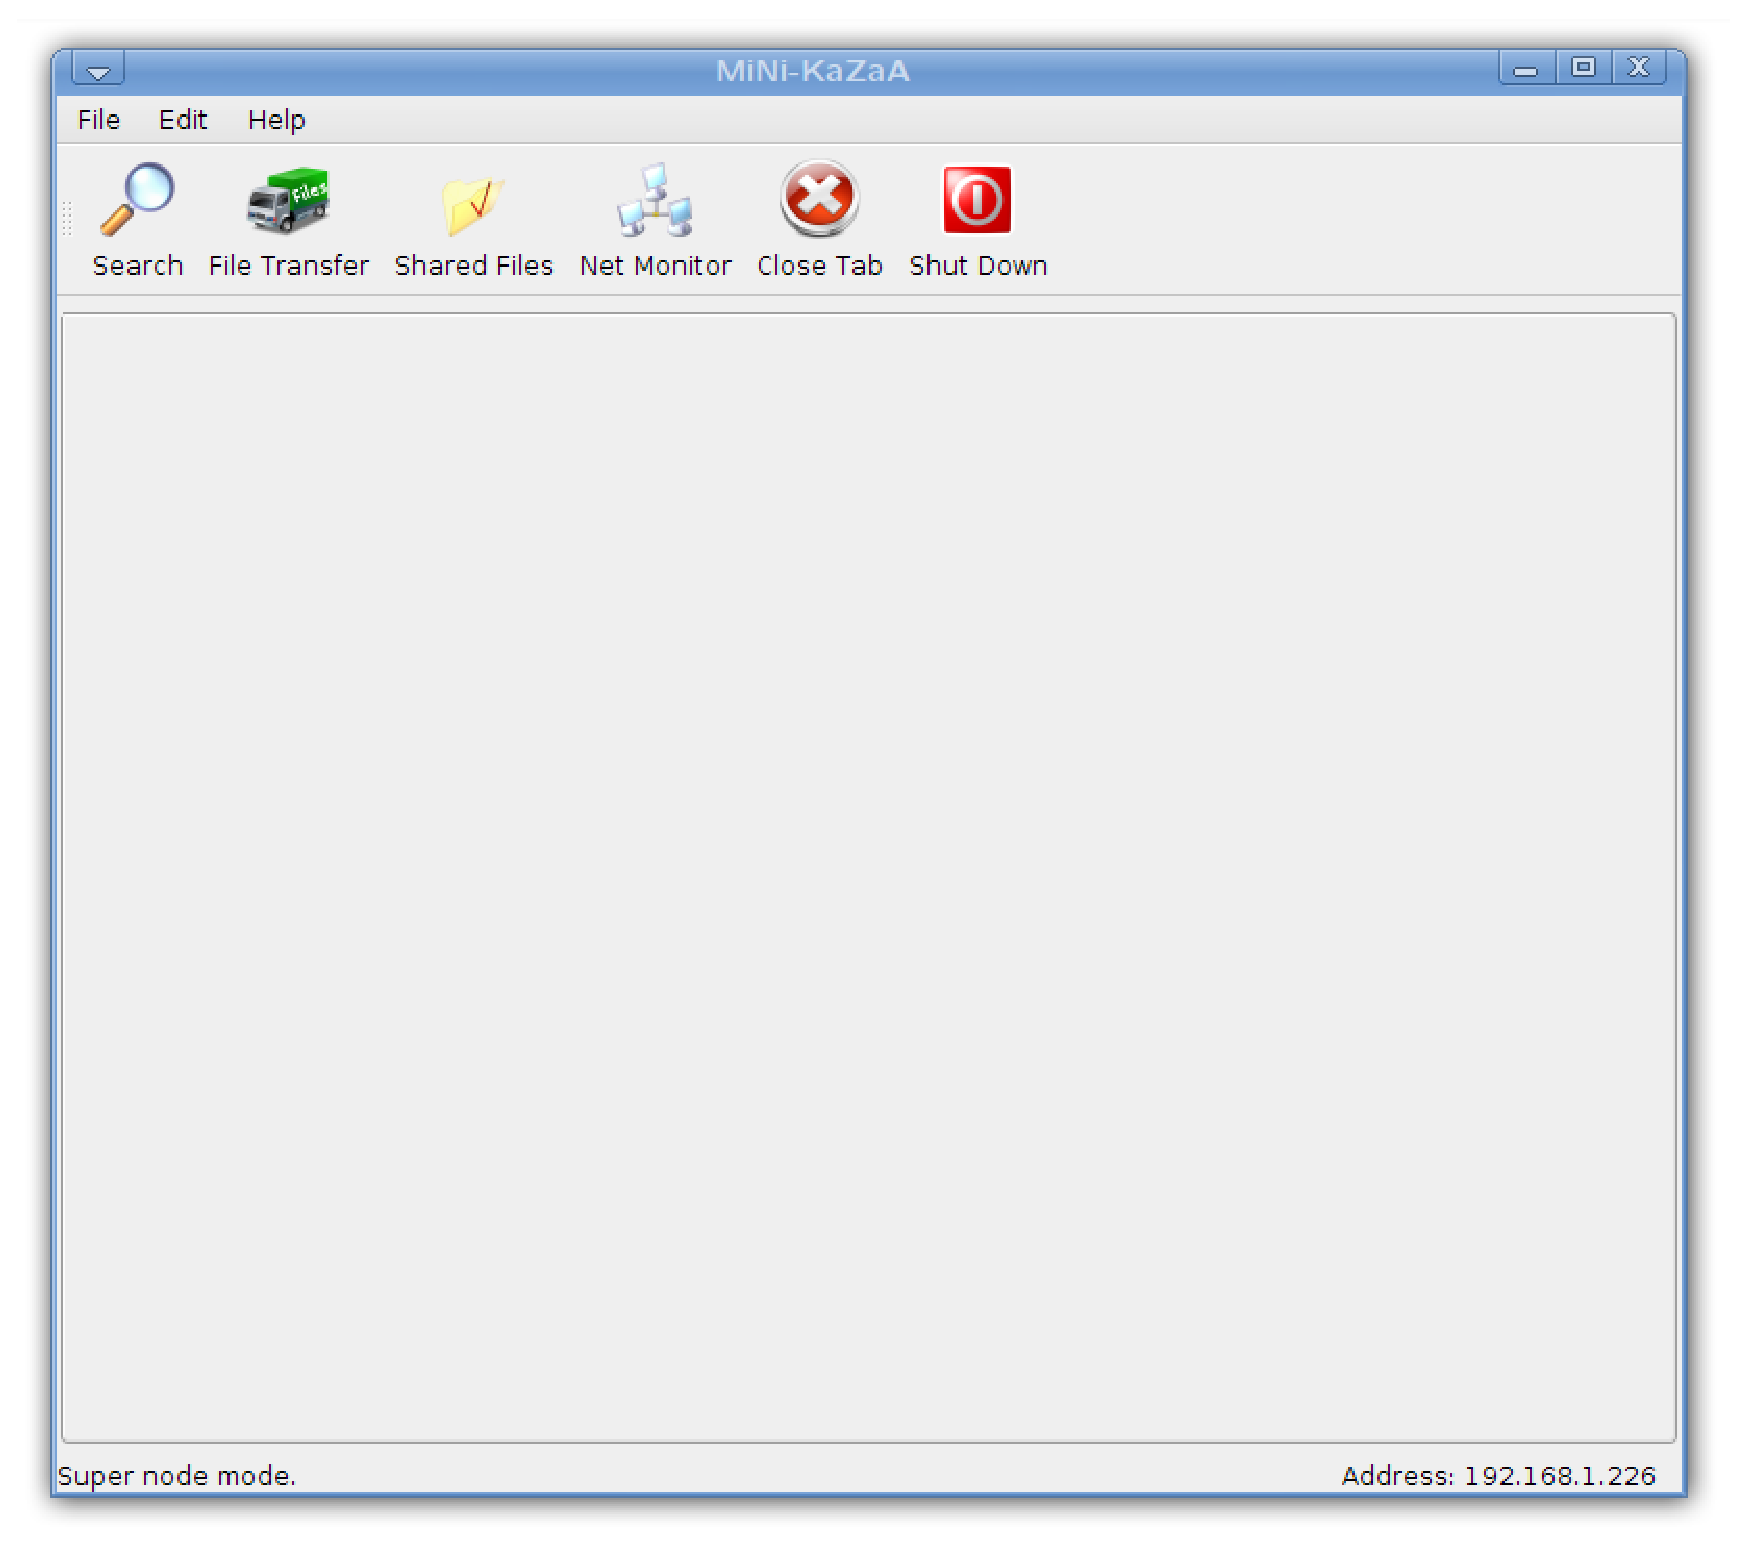
\includegraphics[width=250px,height=225px,bb=14 14 841 737]{images/mini_kazaa_client.eps}
 % mini_kazaa_client.eps: 0x0 pixel, 300dpi, 0.00x0.00 cm, bb=14 14 841 737
 \caption{L'interfaccia grafica principale del client.}
 \label{fig:mini_kazaa_client}
\end{figure}

